% !TEX root =  paper.tex
\section{Approach}

The objective of this chapter is to propose a web form analysis approach 
to automatically create the required DOM markup for accessibility labels. 
The challenges involved in formulating such an approach are as follows. 
First, web pages and forms can have many possible designs and patterns. 
Designing an approach that addresses every potential case is not tractable. 
Therefore, the goal is to first establish an approach that works for many forms while 
remaining generic and robust. This is an important first step since the problem 
of inferring labeling markup has not been addressed before, so the first stage is 
to establish a technique that can be demonstrated to work for many forms, 
after which other corner cases can be addressed by permutations and adjustments 
in subsequent publications. The second challenge is the absence of prior blueprint 
or similar work that can serve as a starting point to formulate the approach. 
It is therefore not readily evident what assumptions are safe to make or what 
sort of analysis steps or general analytic approaches should be utilized to 
address the problem. Accordingly, the approach will be mainly heuristic in 
nature, and its efficacy will ultimately be assessed in the evaluation.  

The overall steps of our approach are as follows. We adopt a strategy of visually 
analyzing the web form to infer labeling associations of form elements, 
and then repairing the DOM such that its markup reflects 
the inferred labels in order to make the form accessible.
The approach begins by loading the web page in an instrumented web browser 
(e.g., via Selenium). 
Next, any forms on the page are then abstracted in preparation for further 
analysis. 
Subsequently, a set of visual cues are constructed from each form. 
These visual cues are then used in the next stage, which is the optimization 
formulation. In this stage, we cast the labeling process as an optimization 
problem, where the minimization and maximization of certain combinations 
of visual cues yield the final form labels. 
Finally, the inferred labels are transformed into standard ARIA accessibility 
attributes and augmented into the DOM of the web page. 

\subsection{Form Abstraction} \label{sec:approach-abs}
The abstraction process extracts essential information from the form by converting 
the form into only two classes of objects: \emph{fields} and \emph{texts}. 
Any other aspect of the form is discarded. 

For fields, we iterate through the possible ways in which form inputs can be 
expressed (e.g., \code{input} elements with various attributes, \code{select} 
elements) and abstract them into a single category of fields.
When it is time to perform the optimization and generate the labels, 
as described in \Cref{sec:approach-opt}, 
working with a single category of fields facilitates a more manageable 
optimization formulation instead of working with a variety of categories. 

For texts, we also perform a similar abstraction. 
Labels in web forms can be expressed using many possible textual elements.  
For example, in \Cref{fig:motivating-example}, \code{p}, \code{div}, and \code{span} 
have been used. We normalize these variations and 
abstract the texts by iterating through the DOM tree and selecting non-empty 
nodes of type \code{\#text}, which represent string literals. 
We note that this is based on a node type, rather than
an element (i.e., tag) type.
This allows more robust abstraction because it captures any text and 
does not make assumptions about how developers choose to place their text.
Regardless of the tag used (e.g., \code{span, div}, attributes), text would still 
be stored in nodes of type \code{\#text}, even for custom HTML elements.
 

\subsection{Labeling Association}  \label{sec:approach-opt}

The labeling association is achieved by gathering visual cues from the abstracted 
form, then using these cues to construct the decision variables that will make 
up the objective functions as well as the constraints. 


\subsubsection{Visual Cues} \label{subsec:cues}
When sighted users browse a web form, they are able to perceive the 
form labels and understand what each field signifies. 
Our goal is to emulate this perception and analysis in 
an automated fashion. 
However, due to the absence of prior analysis approaches for inferring form labels, 
we do not have a reference or general blueprint for what sort of analysis steps may  
be performed to infer the labels or what assumptions are safe to make. 
However, an assumption that is guaranteed to be accurate is that regular users 
take visual information as an input, and build their mental understanding of the 
form as an output. Accordingly, we use this assumption as the basis for analysis. 
That is, we propose a web form analysis approach that emulates users by collecting 
visual information from the form as an input and generate the labeling association 
DOM markup as an output. The next question then becomes what exactly is the kind 
of visual information that should be collected. 

\hl{
Unfortunately, there is no conclusive answer to this question yet. It is not 
definitively known what kind of visual information sighted people intuitively 
use when deciding the labeling in web forms. Furthermore, as mentioned in the 
introduction, web forms can vary greatly in their designs and patterns, which makes 
it difficult to propose a solution that can cover all possible form layouts. 
However, two particular types of 
visual cues may potentially be useful when analyzing web forms to infer label markup, as
will be described in the next paragraph. 
While these visual cues do not cover all possible form designs, they do serve 
as a first step towards solving the problem of accessibility labeling inference. 
We first emphasize an important aspect of the proposed analysis, which is that 
no single cue is sufficient or conclusive on its own. Rather, it is the collective optimization of all possible cue combinations that will yield the final DOM labeling markup. 
This combination of cues mitigates the fragility of depending on a single cue on its own, as will be discussed in \mbox{\cref{subsec:opt}}.
}

The first cue is related to how much an object stands out for a user who is looking at the interface. 
We will refer to this type of information as \emph{visual prominence}. 
It has been shown that users looking at a web page do not pay equal attention 
to all objects on the page~\cite{eraslan2016eye,shen2014webpage}. 
Rather, objects with certain visual characteristics are more likely to gain 
their attention compared to other objects. 
It is therefore likely the case that if we gather the kind of visual characteristics 
that users intuitively focus on, then we would be capturing potentially useful 
cues for analyzing a web form. 
To this end, we capture the following visual characteristics to analyze the 
prominence of various form elements. First, users have been shown to focus on 
objects that are bigger and occupy more space on the screen~\cite{buscher2009you}. 
Accordingly, by capturing size information of form objects, we will be incorporating 
in our model a feature that users tend to focus on when parsing the form. 
Subsequently, existing evidence~\cite{gupta2018saliency} suggests that objects 
with higher contrast tend to receive more focus from users. We therefore add 
this visual cue as well to the list of data to collect from the form. 
Finally, we capture all the aforementioned visual cues into a single metric of 
visual prominence. This metric is constructed by the multiplication of three 
measurements: font size, weight, and contrast. First, each of these values 
are captured for every abstracted form element (as described in 
\Cref{sec:approach-abs}). We then take the maximums 
of each of these values and use that to compute a normalization 
factor. Finally, all visual prominence values are divided by this 
normalization factor to yield the final normalized visual prominence 
values. Only these normalized values are used in the remainder of 
the analysis. More concretely, the visual prominence 
is computed as follows:
\begin{eqnarray}
	p_i =  \left( \frac{s_i}{n_s} \right)  \left( \frac{w_i}{n_w} \right) \left( \frac{c_i}{n_c} \right)
\end{eqnarray}
where $p_i$ is the visual prominence of the $i$-th abstracted form element, 
$s_i$ and $w_i$ are the font size and weight, $c_i$ is the color contrast,  
and $n_s$, $n_w$, $n_c$ are the normalization factors computed from taking 
the maximum value across all abstracted form elements. 
\Cref{fig:illustration}(a) illustrates the nature of the visual prominence cue, 
where the thickness of the line indicates how prominent the various elements are
(i.e., it visualizes the $p_i$ described above). 
We also note how we do not assume some factors are more important than others, and therefore make the unbiased decision do weight all factors equally. 
We can see how the ``free providers..." text receives a lower prominence value compared to the ``Business email" text. 
 
\hl{The second cue is related to the visual \mbox{\emph{layout}} of elements 
on the form. This would provide information on how elements 
are arranged with respect to one another to capture the layout of the form. 
The reason we believe this information would be useful for labels inference 
is because there is evidence~\mbox{\cite{bargas2010simple, wroblewski2008web}} 
that users tend to associate form inputs with their neighboring text fields. 
Accordingly, this information may potentially facilitate emulating 
the kind of visual parsing done by sighted users.  
However, we do emphasize that web forms can vary greatly in their designs and 
layouts, and therefore it is very difficult to propose an inference process that covers 
all possible form layouts. This is the reason that we don't only use the layout 
cue on its own, since it would not necessarily be conclusive on its own. 
Rather, we combine multiple cues in order to reach final labeling decisions. }
We capture this cue by measuring the pair-wise visual geometric Euclidean distance, which is used together with other cues as explained in the previous paragraph. This is done across all abstracted field-text pairs. 
After each pair-wise measurement is collected, we proceed to determine 
the geometric bounds of all measurements. The reason for doing this 
is to normalize the geometric measurements. The reason for doing the normalization is because this cue will be combined with other cues in the objective as well as the constraints 
of the optimization. Accordingly, for the optimization to function properly, 
the geometric measurements must first be normalized, because other cues (e.g., prominence) would have a different range of values 
compared to layout distance, and therefore combining them directly before normalization would skew the optimization towards one cue instead of another. To do this normalization we compute the geometric bound, which is the maximum possible pair-wise 
Euclidean distance for a collection of elements, and is therefore calculated 
once all distances are available. Finally, all distances are divided by 
the geometric bound and the resulting values are the final normalized 
values used in the remainder of the analysis. More concretely, the visual 
layout of the form is a set of data whose elements can be expressed as follows: 
\begin{align}
l_{i,j} = \frac{E(f_i, t_j)}{n_g} 
\end{align}
where $l_{i,j}$ is the pair-wise visual layout cue, 
$E$ is the visual geometric Euclidean distance between 
field $f_i$ and text $t_i$, $n_g$ is the normalization 
factor computed from the geometric bound as explained 
in the previous paragraph. 
\Cref{fig:illustration}(a) illustrates the nature of the visual layout cue, 
where the length of the line visualizes the $l_{i,j}$ values described above. 
The collection of all such pair-wise lines captures the layout of the whole 
form. 

\begin{figure}[t]
	\centering
	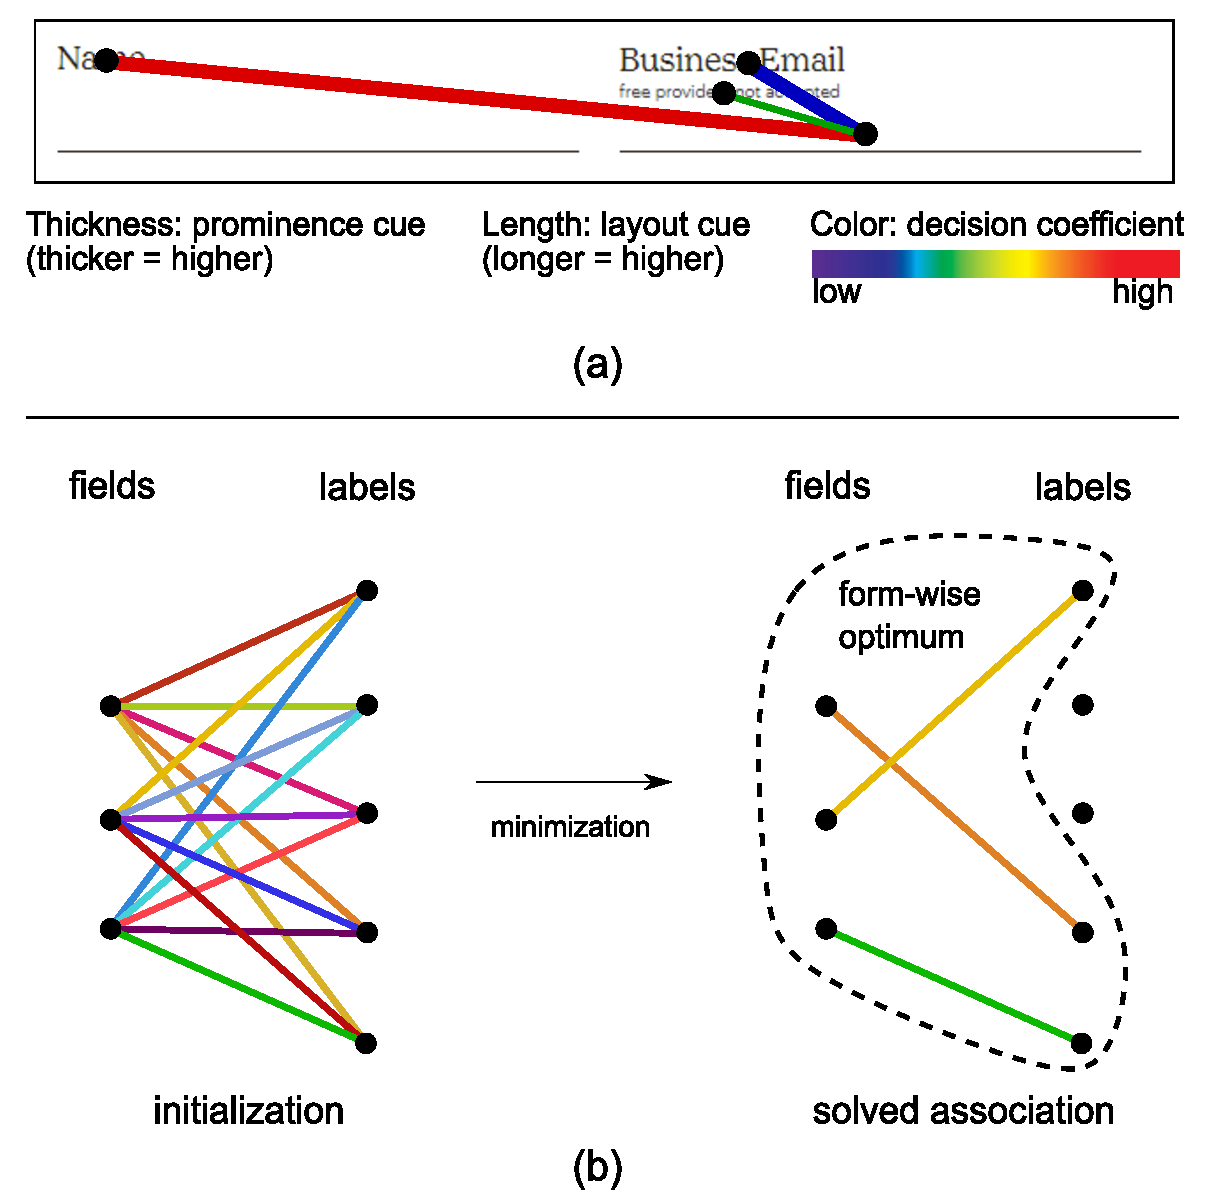
\includegraphics[width=0.86\linewidth]{accessibility_repair/figures/illustration/illustration.pdf}
	\caption{Visualization of (a) the visual cues, and (b) the labeling association. }
	\label{fig:illustration}
\end{figure}

\subsubsection{Decision Variables}
\label{subsec:opt}
Decision variables will be used, in combination with the cues 
gathered from the form, to optimize the assignment of labels. 
The strategy we adopt is to formulate the form labeling analysis 
as a constrained binary program. The rationale for formulating the 
problem in this fashion is as follows. First, the assignment of 
labels must be constrained by other label assignments. That is, 
if a solver has made labeling assignments involving some subset 
of texts, then this should constrain the possible set of texts 
that can be used for remaining labeling assignments for the rest 
of the fields. Furthermore, the labeling assignment can be readily 
expressed as a pair-wise binary function between fields and texts. 
In addition, deciding the form labeling using only individual  
field by field analysis would be a subpar approach. This is because it  
would not consider whether a potential label for a given field might be 
a better match for another field, or whether it was already associated 
with another field. For instance, if field A has equal cue values 
with respect to potential labels X and Y, but field B has optimum 
cue values only with respect to Y, then the optimal decision is to 
assign A to X and B to Y. Having an isolated, field by field analysis 
would not be able to make this decision. In contrast, a global 
combinatorial analysis that takes into account all fields together 
would be a better fit. This is also the reason why the proposed approach 
does not rely on individual cues alone to decide field labeling, but rather 
trades off all cues for all field-label pairs to reach an optimum labeling 
for the form as a whole. For all of the aforementioned aspects, 
a constrained binary program is a potentially suitable approach 
to formulate the labeling problem. 

Accordingly, each decision variable $d_{i,j}$ is a binary value that 
represents the decision of assigning a particular label $t_j$ to a 
particular field $f_i$. \Cref{fig:illustration}(b) illustrates the decision variables. 
On the left hand side of the figure, each line represents one $d_{i,j}$ value. 
Each variable would encode one possibility of labeling. The optimization 
solution, as illustrated on the right hand side of \Cref{fig:illustration}(b), 
represents which decision variables are finally applicable. This is where the 
tradeoff occurs in terms of optimizing various possible combinations of 
visual cues to reach the final labeling. Once all decision 
variables have been determined, the label associated with each field 
is identified. 

\subsubsection{Objective and Constraints}\label{subsec:obj}
In order to create the objective function and constraints, we need to 
consider the kind of labeling markup provided by the ARIA 
standard. This is because the final DOM repair process will include 
generating the necessary markup to convey the inferred labels, and 
this markup has to follow the ARIA standard. The ARIA standard provides 
two types of form labeling: individual and group labels. Individual 
labeling represents the label associated with every single form input 
on its own. For instance, in \Cref{fig:motivating-example}b, individual 
labeling associates the large text area field under 'Message' with the 
label `Message`. For group labeling, consider the two radio option 
fields at the bottom of \Cref{fig:motivating-example}b. The individual 
labels in this case are 'No' and 'Yes', and the group label is `Do 
you have an open ticket`. The strategy we adopt to identify both label 
types is a bottom-up multiple-passes approach. We first infer the 
individual labels, and then use that information to perform another 
pass to identify the group labels. The reason for adopting this 
strategy is that it allows us to optimize the problem for each 
label type separately, and also simplifies group labeling by using 
information from the individual labeling. Therefore, each of these 
label types will have a different objective function and set of constraints. 

Subsequently, each decision coefficient of the optimization is 
calculated as follows: 
\begin{align}
c_{i,j} = \frac{l_{i,j}}{p_i}
\end{align}
where $c_{i,j}$ is the coefficient of the decision variable, $p_i$ is the visual prominence cue, and $l_{i,j}$ is the visual layout cue. The magnitude of each coefficient $c_{i,j}$ describes the 
pair-wise and per-element visual cues. 
The choice of which $i, j$ pairs would constitute a labeling association 
is determined by the objective function and the constraints: 
\begin{equation} \label{eqn:min}
\begin{aligned}
A \; = \; \mathrm{argmin}_{} \; & \sum_{i}\sum_{j} c_{i,j} d_{i,j}   \\
\textrm{s.t.}	\quad & \sum_{j} d_{f_1,j} = 1, \cdots \sum_{j} d_{f_N,j} = 1 \\
							& \sum_{i} d_{i,t_1} \leq 1, \cdots \sum_{i} d_{i,t_M} \leq 1 \\
\end{aligned}
\end{equation}
with $A$ being the labeling associations result. $c$ and $d$ are the coefficients 
and decision variables, respectively, as described in the preceding paragraphs. 
\Cref{fig:illustration}(b) illustrates a number of remarks regarding the above equations. 
First, the color of the lines represent the magnitude of the decision coefficients $c_{i,j}$.  
We can see that the visual cues cover all possible labeling combinations. 
The decision variables then determine which combination of visual cues yields the 
optimal result, as shown on the right hand side of \Cref{fig:illustration}(b). 
We also note that we have two sets of constraints. The first set 
of constraints subjects the optimization to the requirement of finding exactly 
one label. This constraint stems from the ARIA accessibility requirement stating 
that each form field must have a label, and is therefore not assumption or decision 
that we made on our own.  
In \Cref{fig:illustration}(b), only one outgoing line is allowed 
from each field dot. 
Each form field $f$ gets its own constraint equation, containing entries 
for all possible labels. First, this prevents the optimization from yielding the 
trivial solution (i.e., none of the lines in \Cref{fig:illustration}(b) are selected). 
Second, this avoids solutions where only a few fields are 
associated with all labels by virtue of yielding a smaller objective value, 
thereby leaving many other fields without a labeling association. 
For instance, in the solved association in \Cref{fig:illustration}(b) we note that 
the final selection coefficient values are \emph{not} the minimum per each field. That is, 
the final lines on the right hand side are not all blue colored that indicate low coefficient 
values. Rather the final coefficient values are mid-range, illustrating that the 
objective function is seeking the minimum of the whole form, not the individual fields. 
The second set of constraints subjects the optimization to restrictions on the possible 
associations that can be done for text elements. Each text $t$ gets its own 
constraint equation, paired with all possible fields. Paired with the first set 
of constraints, these second constraints enforce a couple of requirements. First, 
that the labeling association for each text entry is optional. That is, it 
encodes the expectation that not every text field present on a form has to be 
a label. We can see this in the solved association in \Cref{fig:illustration}(b) 
where not all the label dots have lines. This is true because forms have many 
texts that are not labels (e.g., descriptions, hints). Furthermore, the constraints 
ensure that each potential label is associated with at most one form field. This enforces the requirement that a solution is not accepted if only a few text elements end up being associated with many fields due to a smaller objective value. 

Once the individual labeling associations are obtained, we proceed to infer the group labeling. First, we discard all texts that have received a labeling association from the individual labeling stage (i.e.,~all $t \in A$). Next, 
our target is to identify groupings of the fields. To achieve this, we take an 
agglomerative clustering approach~\cite{gan_ma_wu_2021}, which is a clustering technique that builds clusters by starting from leaf nodes and than gradually merging groups of nodes. 
The reason for adopting agglomerative clustering is that we use it in a way that enables us to identify groupings without requiring thresholds or parameters. This helps 
in increasing the robustness of analysis, and reduces the often cumbersome manual effort required to tune any parameters. 

We conduct the grouping by first constructing a 
fields distance matrix, whose elements are the visual geometric 
Euclidean distance between each pair of fields. Subsequently, we 
determine the linkage function to be used for the agglomerative 
clustering. This function determines which pair of clusters to 
merge in the next level of agglomeration. For the current task 
of identifying visual groupings, we adopt the single-linkage 
criterion~\cite{gan_ma_wu_2021}. Single-linkage agglomeration 
occurs, in our case, when the minimum visual geometric distance 
between clusters is smallest. 

Accordingly, we run the agglomeration process as per the aforementioned steps. 
We then obtain all heights of the obtained hierarchy of clusters. 
In our case, these heights would signify the progressively increasing visual geometric 
distances between clusters. We then compute the median value of all heights, excluding heights of zero since they don't represent any cluster. This median value is then used as a cutoff to the 
hierarchy of clusters. That is, only clusters whose within-cluster visual geometric distance are below the cutoff are retained. The final result is a set of field groupings.
Once the groupings have been identified, we proceed to infer the labeling associations 
for those groups. We achieve this by performing a second optimization pass and formulate 
the problem as follows:
\begin{equation} \label{eqn:max}
\begin{aligned}
B \; = \; \mathrm{argmax}_{} \; & \sum_{i}\sum_{j} \frac{d_{i,j}}{c_{i,j}}   \\
\textrm{s.t.}	\quad & \sum_{j} d_{f_1,j} \leq 1, \cdots \sum_{j} d_{f_N,j} \leq 1 \\
							& \sum_{i} d_{i,t_1} \leq 1, \cdots \sum_{i} d_{i,t_M} \leq 1 \\
\end{aligned}
\end{equation}
where $B$ is the labeling associations result, 
and $c$ and $d$ are the same variables as those that have 
been used in the first optimization pass, with the exclusion 
of all individual labeling associations that have been obtained 
from that first pass. We make a number of remarks regarding the 
above equations. First, we note that the structure of the 
problem is different from that in the first optimization pass. 
We now have a maximization problem instead of a minimization. 
The rationale for this is as follows. 
First, we note that individual labels are always present while 
group labels may or may not be present~\cite{ARIA}. 
The problem formulation therefore needs to take this into account. 
This brings us to the second observation, which is regarding the 
constraints. In the previous pass, we had constraints to have 
the decision variables finding exactly one label (i.e. the 
equality constraints). In this pass, however, no such requirement 
is made. Instead, we have an upper bound inequality constraint 
on the decision variables pertaining to all form fields (the 
first set of constraints in \Cref{eqn:max}). This encodes the 
fact that group labeling associations may or may not be present 
on a given form, and if it does have one, that its doesn't result 
in a degenerate case where many texts are associated with a given 
field. However, since we now have an upper bound inequality 
instead of an equality constraint, the problem can no longer 
remain a minimization. This is required in order to avoid trivial 
solutions (i.e. zero decision variable selections). Accordingly, 
the problem is formulated as a maximization. The placement of 
the coefficients of decision variables have been adjusted accordingly 
to reflect the change in the objective. However, their computation 
remains the same as before, using the same visual cues we previously 
described. We also note that the second set of constraints 
(pertaining to the text elements) have remained the same as before, 
since we still have the same expectation as the first case that 
not all texts need to partake in a labeling association. 

\subsection{DOM Augmentation Markup}
So far, the form has been abstracted, visual cues generated, and 
the optimizations yielding the labeling associations have been 
solved. At this stage, we perform the final step needed to ensure 
form labeling accessibility, which is repairing the DOM. 
This stage involves transforming the labeling associations into 
ARIA accessibility markups. These markups are finally added to 
the DOM of the page in order to explicitly encode all labels.  

The ARIA standard provides markup for both individual and group 
labels. We will start by describing the encoding for individual 
labels, and then proceed to describe to the case of groups. 
First, we take all the individual labeling associations obtained in 
$A$ (\Cref{eqn:min}).  This provides a mapping of $f_i$ to $t_i$, 
representing pairs of fields and labels, respectively. Next, we 
iterate over each field $f_i$, and examine the associated label 
$t_i$. If the $t_i$ element in the page has an id (i.e. a non-zero 
\code{id} attribute), then we obtain that id. Otherwise, a unique 
random id is generated for that element and added as an \code{id} 
attribute for that element in the DOM. Subsequently, for each field 
$f_i$, we add the \code{aria-labelledby} standard ARIA attribute. 
The value of this attribute is then set to the value of the \code{id} 
attribute of the associated $t_i$, whether that id already exists 
or was generated. If the associated $t_i$ is not an explicit element 
(e.g., the text is contained in an attribute), then we add an 
\code{aria-label} instead of \code{aria-labelledby}, and we set its 
value to be the content of the text, since assigning an id in this 
case is not possible. The ARIA standard allows labeling elements 
using both ids and the actual textual value of the label. 

We then move on to process the group labeling associations 
obtained from $B$ (\Cref{eqn:max}). In this case, the mapping 
result is different from the case of individual labeling 
associations. Here the mapping is from a set of fields 
$\{f_1, \ldots, f_n\}$ to the associated inferred label 
$t_i$. We begin by iterating over each set of fields, and 
examine the associated label. We obtain the id of the associated label, 
or generate a unique one if it does not exist, in the same 
fashion as done in the previous case for individual labels. 
Next, we find the \emph{nearest common ancestor} in the DOM 
for the $\{f_1, \ldots, f_n\}$ set. The reason for doing this 
is the nature of the standard ARIA attribute used to group 
related elements, which is \code{role="group"}. It should 
contain as descendants the group of elements its representing~\cite{aria-group-markup}. 
Accordingly, for the nearest common ancestor node of a set $\{f_1, \ldots, f_n\}$, 
we add the attribute \code{role="group"} to that node to 
communicate the presence of a labeling group. Next, we add 
the \code{aria-labelledby} attribute to the same nearest common 
ancestor node, and set the value of the attribute to the id 
attribute (whether existing or generated) of the mapped label $t_i$ 
associated with the set $\{f_1, \ldots, f_n\}$. Finally, we note 
that the markup repair process can be executed at any time, 
whether on page load, or whenever the DOM of the form is updated 
in dynamic pages. 


\header{Implementation}
We implemented the proposed approach using server-side JavaScript 
(Node). We used the Selenium WebDriver to instrument browsers and 
extract DOM information and computed attributes. To make the study 
replicable, we made available online a link to our data and 
tool~\cite{tool-and-data}, which we called~\toolname (short for 
accessible forms). We used OpenCV~\cite{opencv} for image operations 
and Lpsolve~\cite{lpsolve} to formulate and solve the optimizations. 

